\documentclass[11pt,a4paper]{article}
\usepackage[margin=22mm]{geometry}
\usepackage{fontspec,amsmath,booktabs,graphicx,hyperref}
\setmainfont{STIXGeneral}
\setlength{\emergencystretch}{2em}
\begin{document}
\begin{center}{\Large Topic B: proof routes and acquisition costs}\\[4pt]
Human Compression project\end{center}
The four fixed contracts cover thirty clauses from Buekenhout--Cara (1998),
Cameron--Cara (2002), Archer--Cara--Krempa (2005), and the revised
Garcia-Colin--Leemans manuscript. The common theory is \emph{Forest
coordinates and relative generation}. Its four complete applications
retain the admitted hypotheses, outside theorems, corrections and exclusions.

\paragraph{The complete comparison.}
The whole common paper costs 14,119 characters; the four applications cost
44,942. Three source PDFs contribute 57,539. If $x$ is the unknown original
PDF cost of N001, the complete comparison is
\[R_B=\frac{x+57\,539}{59\,061}.\]
There is no numerical value of $R_B$. The N001 application remains fully
charged. Its authored browser text supplies documentary evidence but is
not substituted for the missing PDF measurement.

\begin{center}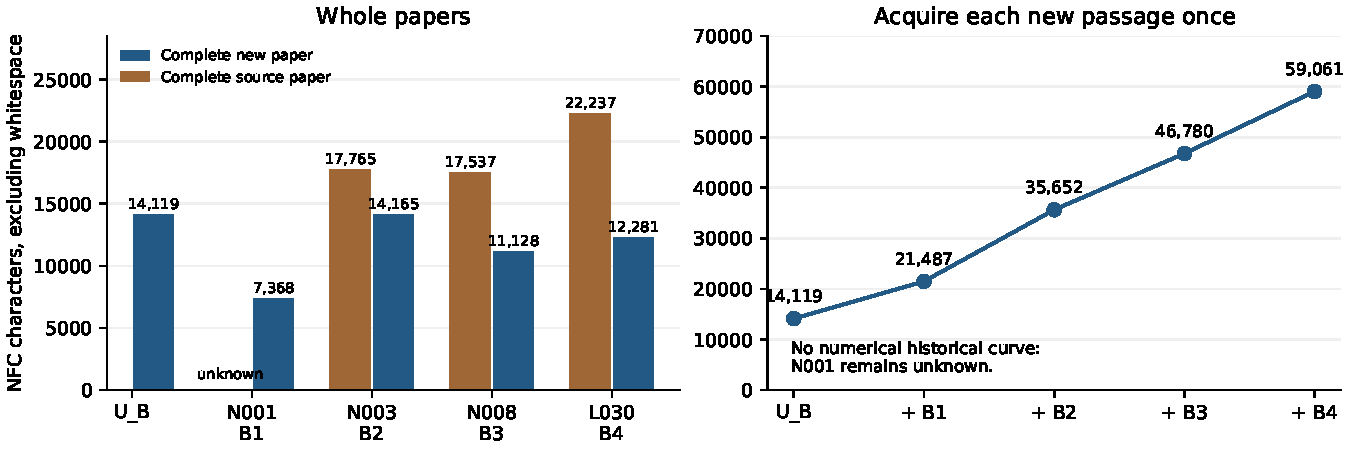
\includegraphics[width=\linewidth]{acquisition.pdf}\end{center}
\noindent The unit throughout this page is NFC characters without whitespace
in the complete extracted PDF text, using the reviewed furniture exclusions
and glyph corrections. Image and expanded outside-proof costs remain unknown.

\paragraph{After acquiring the whole common theory.}
The following admitted factors divide the complete source paper by its
complete application. They do not discount the umbrella in the overall
comparison or charge it again at each application.
\begin{center}\begin{tabular}{lrrr}\toprule
Source / application & Source & Application & Conditional factor\\\midrule
N001 / B1 & unknown & 7,368 & unknown\\
N003 / B2 & 17,765 & 14,165 & 1.254\\
N008 / B3 & 17,537 & 11,128 & 1.576\\
L030 / B4 & 22,237 & 12,281 & 1.811\\
\bottomrule\end{tabular}\end{center}
This proof edition has no required mathematical program dependency.
Validation infrastructure and the six scoped Lean declarations are separately
inventoried; they are not claims of complete formalization.
\newpage
\paragraph{One explicit acquisition order.}
Start with the complete $U_B$, then acquire B1, B2, B3 and B4. Let $K_i$
be the union of passage owners paid through stage $i$. The added cost is
$c(K_i\setminus K_{i-1})$; every complete local paper, including context
and references, belongs to $K_i$. Recorded prerequisites already in
$K_{i-1}$ are not charged again. The table is an exact union calculation,
not a proposed shortest proof or an estimate of time spent.
\begin{center}\begin{tabular}{lrrr}\toprule
Paper added & New cost & Cumulative & Prior passages used\\\midrule
U\_B & 14,119 & 14,119 & ---\\
B1 & 7,368 & 21,487 & 6,995\\
B2 & 14,165 & 35,652 & 10,208\\
B3 & 11,128 & 46,780 & 6,450\\
B4 & 12,281 & 59,061 & 5,314\\
\bottomrule\end{tabular}\end{center}
The last column counts the already paid passages appearing in that
application's recorded proof route. It is not an extra subtraction from the
new cost. Every historical cumulative stage is symbolic: $x$, then
$x+17\,765$, $x+35\,302$, and $x+57\,539$.

\paragraph{What the paired graph explains.}
The offline reader selects a whole contract or any of its thirty clauses.
Arrows run from prerequisite to use. It offers a compact named-result view
and an expanded proof-branch view. Selecting a box gives the precise source
or current proof location, its paid passages and retained assumptions.
Comparison, attribution and verification links are displayed separately
from proof prerequisites. The five repaired documentary interfaces in the
accepted logical revision remain in force, including the implicit Kneser
connectedness premise and the two Whiston inputs' retained classification
provenance.

The graph contains 73 historical nodes, 85 new nodes, 19 retained external
inputs and seven verification components: 184 nodes and 348 fine edges.
These categories include definitions, statements and proof branches. They
are not comparable counts of results, and no node-count factor is reported.
There are 217 disjoint spans with 214 text owners. Parent boxes and proof
branches can share owners: box costs overlap, while totals count each passage
once. Statement-only source passages are labeled as such; a proof charged
elsewhere does not become an additional cost here.

\paragraph{Result routes and whole papers answer different questions.}
A selected prerequisite union explains which recorded arguments support a
result. It can omit context that is still paid in the complete-paper total.
Neither this union nor a graph traversal is a minimum proof cost. The full
umbrella remains paid within Topic B, independently of other topics.
External proofs, missing original-PDF text and unextracted graphics remain
unknown in both views.

\paragraph{Reproduction and scope.}
The standalone HTML retains all thirty clause mappings and all fine edges;
its JSON files bind the reviewed graph, corrected ownership layer and
admitted measurements. The generated figures and this reader are derived
explanations. They do not change any mathematical contract, source credit,
question count or previously admitted factor. A separate checker verifies
complete owner unions, input hashes and the absence of an invented historical
curve; the UI harness tests all contract and clause routes. No primary-source
text or images are distributed in this reader.
\end{document}
